\documentclass[conference]{IEEEtran}
\IEEEoverridecommandlockouts
\usepackage{cite}
\usepackage{amsmath,amssymb}
\usepackage{graphicx}
\usepackage{booktabs}
\usepackage{algorithm}
\usepackage{algpseudocode}
\usepackage{xcolor}
\usepackage[hidelinks]{hyperref}
\graphicspath{{figures/}}
% Let floats fill more of a page so they stay close to the text that cites them.
\renewcommand{\topfraction}{0.9}
\renewcommand{\dbltopfraction}{0.9}
\renewcommand{\textfraction}{0.07}
\renewcommand{\floatpagefraction}{0.8}
\renewcommand{\dblfloatpagefraction}{0.8}
\setcounter{topnumber}{3}
\setcounter{dbltopnumber}{2}
\setcounter{totalnumber}{5}

\begin{document}

\title{Concept Drift Detection in Social Media Streams:\\
Informed Ageing Naive Bayes with an Error-Based ADWIN Detector%
\thanks{Team 18, IOE413 Streaming Data Analytics mini project, Semester 7.}}

\author{
\IEEEauthorblockN{Bichu Devnarayan}
\IEEEauthorblockA{\textit{Roll No. 2023BCS0102}\\
\textit{IIIT Kottayam}, India}
\and
\IEEEauthorblockN{Albin John}
\IEEEauthorblockA{\textit{Roll No. 2023BCD0005}\\
\textit{IIIT Kottayam}, India}
\and
\IEEEauthorblockN{Sarthak}
\IEEEauthorblockA{\textit{Roll No. 2023BCS0068}\\
\textit{IIIT Kottayam}, India}
\and
\IEEEauthorblockN{Aswin Paramesh}
\IEEEauthorblockA{\textit{Roll No. 2023BCD0024}\\
\textit{IIIT Kottayam}, India}
}

\maketitle

\begin{abstract}
Sentiment classifiers deployed on social media streams degrade when the stream changes, a
phenomenon known as concept drift. Iosifidis et al.\ adapt an ageing Multinomial Naive Bayes
(MNB) classifier when a vocabulary-based detector signals change. Such a detector, however,
only sees changes in \emph{which words} are used; it cannot see a change in \emph{what they
mean}. We reproduce the informed ageing MNB on the Sentiment140 stream and add an ADWIN
detector on the prequential error stream, fused with the vocabulary detector. The system runs
end to end on Apache Kafka and Spark Structured Streaming, with metrics in InfluxDB and live
dashboards in Grafana. On controlled drift scenarios with known drift points, ADWIN detects a
label flip after 39 instances instead of 3{,}999, recovers in 3{,}183 instances instead of
8{,}204 and raises accuracy from 71.0\% to 73.8\% (5 seeds). When only one topic's meaning
changes, the vocabulary detector misses the drift in 2 of 5 runs while ADWIN detects all of
them. On the real streams the enhancement improves accuracy from 80.8\% to 81.3--81.7\% (DS1)
and from 83.0\% to 83.7--84.1\% (DS2), adding about 10\,ms of model time per 1{,}000 tweets
in the streaming pipeline.
\end{abstract}

\begin{IEEEkeywords}
concept drift, data streams, sentiment analysis, ADWIN, naive Bayes, Apache Kafka, Spark
Structured Streaming
\end{IEEEkeywords}

\section{Introduction}
Opinions on social media form an unbounded, non-stationary stream: topics come and go,
vocabulary evolves and real-world events shift the sentiment towards an entity. Bechini et
al.\ show that a stance classifier trained once and deployed on Twitter loses accuracy as
events change the discussion, and that adaptive learning schemes recover it~\cite{bechini2021}.
In streaming terms this is \emph{concept drift}: the joint distribution $P(X, y)$ changes
over time~\cite{gama2014}. A change in $P(X)$ alone (new words, new topics) is \emph{virtual}
drift; a change in $P(y\,|\,X)$ (the same words now signal a different class) is \emph{real}
drift, and only real drift necessarily hurts a classifier. The velocity of such a stream rules
out periodic batch retraining: the classifier has to learn online, one tweet at a time, and
decide on the fly when to forget.

\textbf{Problem statement.} Iosifidis et al.\ propose \emph{informed} adaptation for sentiment
streams~\cite{iosifidis2017}: an ageing MNB classifier forgets old observations through an
ageing factor $\lambda$, and a vocabulary-based change detector decides when to forget faster
or rebuild. The detector compares the vocabulary of recent tweets with that of past tweets, so
it reacts to virtual drift by construction, and the authors note that it reacts with delay
because vocabularies of different topics overlap~\cite{iosifidis2017}. A drift in meaning with
an unchanged vocabulary, such as a word that changes polarity after an event, is invisible to
it. We ask whether monitoring the classifier's own errors closes that gap, at what cost, and
whether it holds up in a real streaming pipeline. Our contributions are:
\begin{itemize}
\item A reproduction of the informed ageing MNB with all five $\lambda$ strategies on the
  Sentiment140 stream and a volatile variant, including fixes to the detector that the paper
  leaves underspecified (Section~\ref{sec:enhancement}).
\item An enhancement that adds ADWIN~\cite{bifet2007} on the prequential error stream, with four
  fusion modes and a rebuild reaction on the post-drift window.
\item Controlled drift scenarios with known drift points, following Costa et
  al.~\cite{costa2014}, including a label-flip scenario that isolates real drift with an
  unchanged vocabulary, and an evaluation of detection delay, false alarms, misses, recovery
  time and cost over 224 runs.
\item An end-to-end streaming system on Kafka, Spark, InfluxDB and Grafana that runs both models
  side by side on identical data.
\end{itemize}

\section{Related Work}
\subsection{Base Papers}
\textbf{Iosifidis et al.~\cite{iosifidis2017} (baseline).} \emph{Question:} how can a sentiment
classifier adapt to change in an opinionated stream? \emph{Data:} Sentiment140~\cite{go2009},
1.6M tweets from April to June 2009, and a more volatile variant. \emph{Model:} the ageing MNB
of Wagner et al.~\cite{wagner2015}, whose ageing factor $\lambda$ is tuned online by five
strategies whenever a vocabulary-based detector signals change. \emph{Metrics:} prequential
accuracy over time and overall. \emph{Findings:} informed adaptation beats both never forgetting
and forgetting at a fixed rate (about 78\% vs 73\% on DS1).

\textbf{Costa et al.~\cite{costa2014} (drift scenarios).} \emph{Question:} how do learning
strategies cope with different kinds of drift on Twitter? \emph{Data:} about 10k English tweets
re-timestamped to simulate sudden, gradual, incremental and recurring drift. \emph{Model:} SVM on
bag of words with time-window, ensemble and incremental learning. \emph{Metrics:} precision,
recall, F1. \emph{Findings:} no single strategy is best for every drift type.

\textbf{Bechini et al.~\cite{bechini2021} (motivation).} \emph{Question:} how should a Twitter
classifier adapt when real-world events change the stream? \emph{Data:} several years of Italian
vaccination tweets. \emph{Model:} TF-IDF with a linear SVM under static, retraining, ensemble and
event-based schemes. \emph{Metrics:} accuracy and macro F1. \emph{Findings:} event-driven drift
degrades a static model; adaptive schemes recover the lost accuracy.

\subsection{Drift Detection and Streaming Systems}
Gama et al.\ survey drift detection and adaptation and distinguish \emph{blind} adaptation
(forgetting at a fixed rate) from \emph{informed} adaptation that reacts to detected
change~\cite{gama2014}. ADWIN keeps an adaptive window over a numeric stream and cuts it when two
sub-windows have significantly different means, with bounds on false positives and
negatives~\cite{bifet2007}; on a 0/1 error stream it is a standard error-rate detector. Bifet and
Frank study Twitter sentiment as a stream~\cite{bifet2010}. Kafka provides an ordered, replayable
log~\cite{kreps2011}, Spark Structured Streaming processes it in micro-batches~\cite{armbrust2018}
and River provides online learning and drift detectors in Python~\cite{montiel2021}.

\subsection{Gap}
The baseline's detector watches only the input distribution. It is blind to real drift that
keeps the vocabulary, and it can only react once per check window $w$ (24k tweets on DS1). None
of the base papers combines an input-based and an error-based detector, measures detection
delay and recovery against known drift points, or runs the method on a live streaming stack.

\section{System Architecture}\label{sec:architecture}
Fig.~\ref{fig:architecture} shows the pipeline and every tool in it. \emph{Data preparation}
turns the Sentiment140 CSV into parquet streams in timestamp order (DS1, DS2 and the controlled
scenarios). A Python \emph{producer} replays a stream at a chosen rate into the Kafka topic
\texttt{tweets} as JSON; the topic has a single partition because Kafka orders messages only
within a partition and the models must see tweets in arrival order. \emph{Spark Structured
Streaming} reads the topic in micro-batches of at most 1{,}000 tweets; the executors parse the
JSON and tokenise each tweet in a UDF that calls the same function as the offline runner. Ageing
MNB is sequential and stateful, so each micro-batch is collected to the \emph{driver} inside
\texttt{foreachBatch}, where the baseline and the enhanced model process it side by side, one
tweet at a time in Kafka offset order (predict, then learn). After every batch the driver writes
per-model metrics, pipeline metrics and drift events to \emph{InfluxDB} in one request, and a
provisioned \emph{Grafana} dashboard plots them live, with every detected drift as an
annotation. Kafka, Spark (master and worker), InfluxDB, Grafana and a Kafka UI run in Docker
Compose.

All models, detectors and metrics live in one Python package (\texttt{core/}) that has no
dependency on Spark. The streaming consumer and an \emph{offline runner} both build models from
the same specifications, so the 224-run experiment grid can replay the parquet streams without
Kafka at 37--46k tweets/s while producing the same predictions as the live system.

\begin{figure*}[!t]
\centering
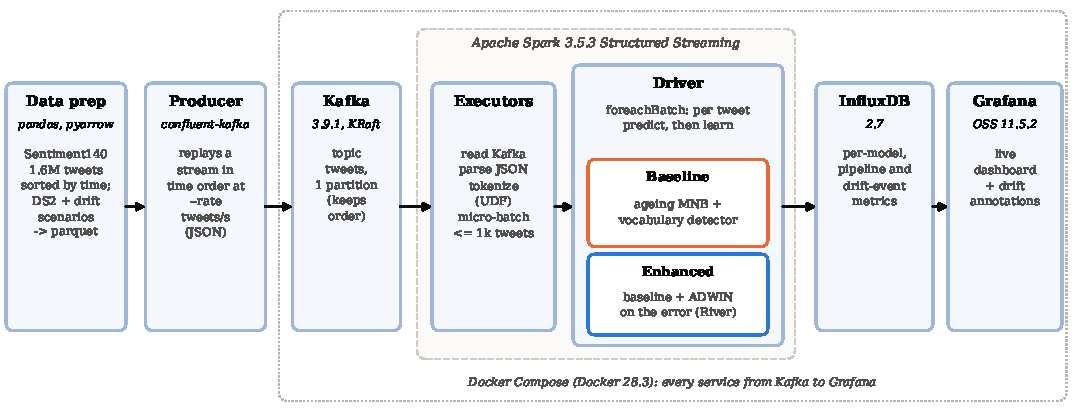
\includegraphics[width=\textwidth]{fig0_architecture.pdf}
\caption{System architecture with every tool and the data flow. The driver runs the baseline and
the enhanced model on identical micro-batches and writes metrics and drift events to InfluxDB.}
\label{fig:architecture}
\end{figure*}

\section{Proposed Enhancement}\label{sec:enhancement}

\subsection{Reproduced Baseline: Informed Ageing MNB}
Following~\cite{wagner2015,iosifidis2017}, the model stores for every class $c$ its count $N_c$
and last observation time $t^c_{lo}$, and for every (word, class) pair its count $N_{wc}$ and
last time $t^{w,c}_{lo}$. At time $t$ counts are aged on read:
\begin{align}
P^t(c) &\propto N_c\, e^{-\lambda (t - t^c_{lo})}, \label{eq:prior}\\
P^t(w\,|\,c) &= \frac{N_{wc}\, e^{-\lambda (t - t^{w,c}_{lo})} + \alpha}
  {\sum_{j} N_{jc}\, e^{-\lambda (t - t^{j,c}_{lo})} + \alpha |V|}, \label{eq:likelihood}
\end{align}
with Laplace smoothing $\alpha = 1$, scores in log space and unseen words ignored; $\lambda = 0$
gives the accumulative MNB. Every $w$ instances the vocabulary detector compares, per class,
the vocabulary $V_{sl}$ of the latest window with a reference vocabulary $V$ by
$\mathrm{precision} = |V_{sl} \cap V| / |V|$, and flags a change if the precision leaves
$\mu \pm \alpha_d \sigma$ ($\alpha_d = 1.8$) and a warning at $\beta \sigma$ ($\beta = 0.334$),
where $\mu, \sigma$ are the moving mean and standard deviation of past checks. On a change, one
of five strategies adapts the model~\cite{iosifidis2017}: \emph{SlowIncreaseUpToALimit}
($\lambda \mathrel{+}= c$ up to $\lambda_{max}$), \emph{SlowIncreaseFastReset} (the same, reset
after one window at $\lambda_{max}$), \emph{FastSetFastReset} ($\lambda = \lambda_{max}$ for one
window), \emph{FastSetSlowDecrease} ($\lambda = \lambda_{max}$, then $-5\%$ per window) and
\emph{Rebuild} (a new model on the instances buffered since the warning), each with
$\lambda_0 = 0$ (\emph{-Zero-}) or $\lambda_0 > 0$ (\emph{-Init-}).

Two details are not fixed by the paper and matter in practice. An \emph{accumulated} reference
vocabulary grows while $V_{sl}$ does not, so precision falls steadily (0.45 to 0.10 over 80k
stable tweets) and the detector fires constantly; we use the \emph{previous window} as
reference, which makes the statistic stationary. Moving statistics over 10 checks produced many
false alarms; 20 checks remove them on our sudden-drift scenario.

\subsection{Enhancement: ADWIN on the Prediction Error}
Prequential evaluation tests each tweet before learning it, so the model observes the error
$e_i = [\hat{y}_i \neq y_i]$ for free. We feed $e_i$ to ADWIN~\cite{bifet2007,montiel2021} with
$\delta = 0.01$ and count only cuts after which the error rate went \emph{up}. Because ADWIN
watches $P(y\,|\,X)$ through the errors, it sees real drift regardless of the vocabulary, and
because it updates on every tweet it is not tied to the check window $w$.

The two detectors drive two channels (Algorithm~\ref{alg:enhanced}): vocabulary signals go to the
$\lambda$ strategy as in the baseline, ADWIN signals trigger a \emph{rebuild on ADWIN's post-drift
window} (its current width, at least 100 instances). The fusion mode decides how they combine:
\emph{vocab\_only} (the baseline), \emph{adwin\_only}, \emph{or} (both channels act; our main
model) and \emph{and} (a signal counts only if the other detector fired within $w$ instances).
Each channel has its own cooldown of 2{,}000 instances, and ADWIN starts after a 1{,}000-instance
warm-up.

\textbf{Why these choices.} Three came from failures we observed. (i) Resetting ADWIN after
every rebuild blinded it: a vocabulary false alarm one instance before the drift left a fresh
ADWIN without a record of the normal error level, so ADWIN is never reset; it drops its old
window itself when it fires. (ii) A shared cooldown let that same false alarm swallow ADWIN's
detection 64 instances later, hence per-channel cooldowns. (iii) A minimum rebuild size of
1{,}000 padded the rebuild with old-concept tweets because ADWIN fires within tens of instances;
a minimum of 100 cut recovery on the label flip from 5{,}626 to 3{,}023 instances.

\begin{algorithm}[t]
\caption{Enhanced informed ageing MNB, one prequential step}\label{alg:enhanced}
\begin{algorithmic}[1]
\Require tweet $(d, y, t)$, model $M$, vocabulary detector $D_V$, ADWIN $D_A$, strategy $S$
\State $\hat{y} \gets M.\textsc{predict}(d, t)$; \quad $M.\textsc{learn}(d, y, t)$
\State append $(d, y, t)$ to the recent buffer $B$
\If{$i \geq$ warm-up \textbf{and} $D_A.\textsc{update}([\hat{y} \neq y])$ signals a rise}
  \If{fusion $\neq$ \textit{and} \textbf{or} $D_V$ fired within $w$}
    \If{ADWIN channel not cooling down}
      \State $M \gets$ new model trained on the last $\max(D_A.\mathrm{width}, 100)$ items of $B$
    \EndIf
  \EndIf
\EndIf
\If{fusion $\neq$ \textit{adwin\_only} \textbf{and} $D_V.\textsc{add}(d, y)$ completes a window}
  \State $s \gets$ signal of $D_V$ \Comment{none / warning / change}
  \If{fusion $=$ \textit{and}} $s \gets$ change iff $s \neq$ none and $D_A$ fired within $w$ \EndIf
  \State apply $S.\textsc{onCheck}(s)$ to $M$ \Comment{set $\lambda$ or rebuild}
\EndIf
\end{algorithmic}
\end{algorithm}

\section{Implementation}

\subsection{Dataset and Streams}
\textbf{DS1} is Sentiment140~\cite{go2009}: 1.6M tweets from 6 April to 25 June 2009 with
emoticon-derived labels. The file is sorted by label, so we sort by timestamp (Fig.~\ref{fig:ds1}).
The last positive tweet is instance 1{,}324{,}774; from 1{,}324{,}775 the stream is all negative,
matching the paper's change point at about 1{,}326{,}000. 1{,}685 tweet ids occur twice with
opposite labels (label noise); we keep them in DS1 and DS2.
\textbf{DS2} is the paper's volatile variant: removing class fractions from six equal segments of
the pre-change stream gives exactly the paper's 1{,}073{,}065 tweets (378{,}288 positive), with
the positive share swinging 68/27/70/17/56/28\% and then 0\%. The paper does not specify which
instances it removed, so the segment pattern is our own.
\textbf{Controlled scenarios} re-timestamp real tweets (one per second, 80{,}000 per stream)
following Costa et al.~\cite{costa2014}, with keyword-defined topics A (work/school) and B
(music/movies), each balanced 50/50 by class and without the duplicated ids: \emph{sudden} (A to
B at 40k), \emph{gradual} (B's share rises from 0 to 1 over 30k--50k), \emph{recurring} (A, B, A,
B every 20k), \emph{prior shift} (50\% to 10\% positive at 40k), \emph{label flip} (every label
inverts at 40k; $P(X)$ and $P(y)$ unchanged) and \emph{label flip (topic)} (only topic A's labels
invert). Each is generated with 5 seeds and a file listing its true drift points.

\begin{figure}[!t]
\centering
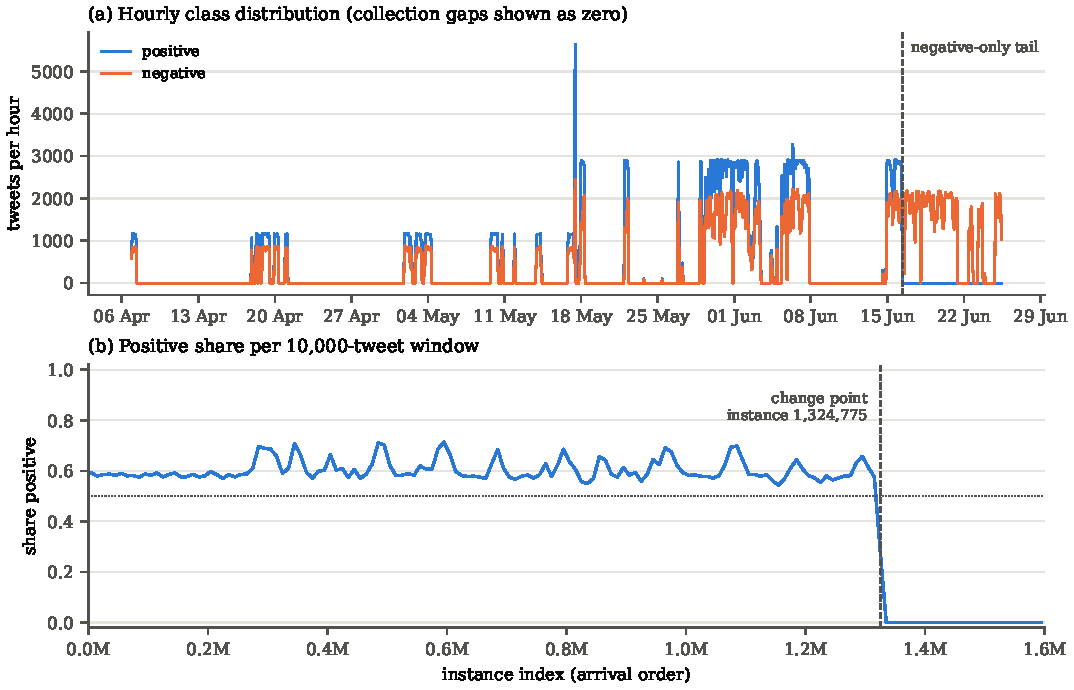
\includegraphics[width=\columnwidth]{ds1_hourly_class_distribution.pdf}
\caption{DS1: (a) hourly class counts (cf.\ Fig.~1a of~\cite{iosifidis2017}); (b) positive
share per 10k tweets with the natural change point.}
\label{fig:ds1}
\end{figure}

\subsection{Tools and Versions}
Table~\ref{tab:tools} lists the tools. The Spark image extends \texttt{apache/spark:3.5.3} with
the Kafka connector jars and the Python packages the driver needs; the project directory is
mounted into both Spark containers so they import the same \texttt{core/} package.

\begin{table}[t]
\centering
\footnotesize
\caption{Tools and versions.}
\label{tab:tools}
\resizebox{\linewidth}{!}{%
\begin{tabular}{lll}
\toprule
Tool & Version & Role \\
\midrule
Python & 3.12.4 (host), 3.10 (Spark) & all code \\
Apache Kafka (KRaft) & 3.9.1 & ordered, replayable tweet log \\
confluent-kafka & 2.15.1 & producer client \\
Apache Spark + spark-sql-kafka & 3.5.3 & Structured Streaming consumer \\
River & 0.26.1 (host), 0.22.0 (Spark) & ADWIN detector \\
InfluxDB / influxdb-client & 2.7 / 1.50.0 & time-series metric store \\
Grafana OSS & 11.5.2 & live dashboard, annotations \\
Docker / Compose & 28.3.2 / 2.39.1 & deployment of all services \\
pandas / pyarrow & 3.0.6 / 25.0.1 & data preparation, parquet \\
scikit-learn / pytest & 1.9.1 / 9.1.1 & reference MNB, 46 unit tests \\
matplotlib & 3.11.2 & figures \\
\bottomrule
\end{tabular}}
\end{table}

\subsection{Key Configuration Choices}
\emph{Time unit.} We measure $t$ in hours from the tweet timestamp. With the paper's
$\lambda = 0.2$ per \emph{instance}, a word unseen for 100 tweets keeps $e^{-20}$ of its weight
and pre-change accuracy on DS1 drops to 68.0\%; per hour the model behaves as in the paper.
\emph{Normaliser.} The sum in the denominator of \eqref{eq:likelihood} runs over the whole
vocabulary; we cache it per class relative to a reference time, update a word's term in $O(1)$
and rescale before $e^{\lambda(t - t_{ref})}$ can overflow, so a prediction costs $O(|d|)$. Unit
tests check the cache against the literal equations and the accumulative model against
scikit-learn's \texttt{MultinomialNB}.
\emph{Streaming.} One Kafka partition; micro-batches of at most 1{,}000 tweets (5{,}000 for the
highest rates); a fresh Spark checkpoint per consumer start, because the model state lives in
driver memory; model state kept for the last three producer runs.
\emph{Models.} The baseline uses Table~1 of~\cite{iosifidis2017} ($w = 24$k on DS1, 22k on DS2;
$\lambda_{max} = 0.5$ for the SlowIncrease strategies, missing from the table); scenarios use
$w = 4{,}000$. ADWIN $\delta = 0.01$ and $\alpha_d = 1.8$ come from a sweep of $\delta \in
\{0.002, 0.01, 0.05\}$ and $\alpha_d \in \{1.5, 1.8, 2.5\}$ over all scenarios and 3 seeds
(432 runs): every enhanced setting beat every baseline setting, and $\delta = 0.01$ gave the
fewest false alarms at equal accuracy.

\begin{figure*}[!t]
\centering
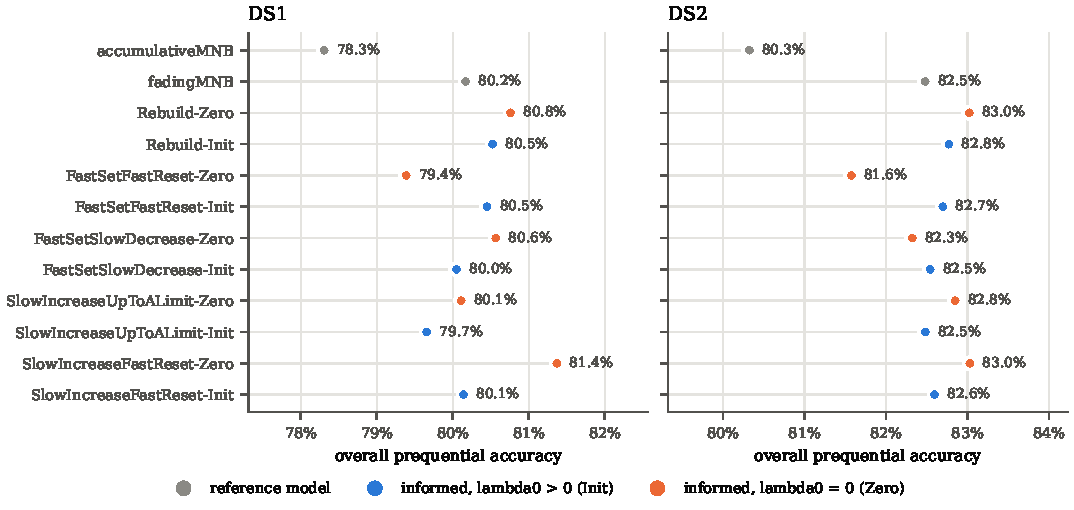
\includegraphics[width=\textwidth]{baseline_overall_accuracy.pdf}
\caption{Baseline reproduction: overall accuracy of the reference models and all informed
strategies on DS1 and DS2 (Table~1 parameters of~\cite{iosifidis2017}).}
\label{fig:baseline}
\end{figure*}

\begin{table*}[t]
\centering
\footnotesize
\caption{Prequential accuracy (\%) per stream; scenarios: mean $\pm$ std over 5 seeds.}
\label{tab:accuracy}
\resizebox{\linewidth}{!}{%
\begin{tabular}{lrrrrrrrr}
\toprule
Model & DS1 & DS2 & label flip & label flip (topic) & prior shift & sudden & gradual & recurring \\
\midrule
accumulative MNB & 78.3 & 80.3 & 53.3 $\pm$ 0.1 & 62.3 $\pm$ 0.1 & 80.3 $\pm$ 0.1 & 73.9 $\pm$ 0.1 & 73.8 $\pm$ 0.1 & 74.0 $\pm$ 0.1 \\
fading MNB & 80.2 & 82.5 & 55.7 $\pm$ 0.1 & 62.3 $\pm$ 0.1 & 80.1 $\pm$ 0.1 & 73.8 $\pm$ 0.1 & 73.8 $\pm$ 0.1 & 73.9 $\pm$ 0.1 \\
baseline: Rebuild-Zero & 80.8 & 83.0 & 71.0 $\pm$ 1.0 & 63.1 $\pm$ 0.4 & 81.6 $\pm$ 0.3 & 73.9 $\pm$ 0.2 & 73.7 $\pm$ 0.1 & 73.3 $\pm$ 0.2 \\
baseline: SlowIncreaseFastReset-Zero & 81.4 & 83.0 & 54.5 $\pm$ 0.6 & 62.2 $\pm$ 0.1 & 80.2 $\pm$ 0.1 & 73.7 $\pm$ 0.1 & 73.7 $\pm$ 0.1 & 73.8 $\pm$ 0.1 \\
enhanced: ADWIN only & 81.6 & 84.1 & 74.3 $\pm$ 0.1 & 64.0 $\pm$ 0.2 & 80.3 $\pm$ 0.1 & 73.9 $\pm$ 0.1 & 73.8 $\pm$ 0.1 & 73.7 $\pm$ 0.3 \\
enhanced: OR & 81.3 & 83.7 & 73.8 $\pm$ 0.3 & 63.5 $\pm$ 0.5 & 81.6 $\pm$ 0.3 & 73.9 $\pm$ 0.2 & 73.7 $\pm$ 0.1 & 73.2 $\pm$ 0.1 \\
enhanced: AND & 81.7 & 84.0 & 73.4 $\pm$ 0.9 & 63.8 $\pm$ 0.5 & 80.3 $\pm$ 0.1 & 73.9 $\pm$ 0.1 & 73.8 $\pm$ 0.1 & 73.6 $\pm$ 0.3 \\
\bottomrule
\end{tabular}}
\end{table*}


\section{Experimental Setup and Results}

\subsection{Setup and Metrics}
The grid evaluates 7 models on 8 streams, with the 6 scenarios generated 5 times each (224 runs):
the accumulative MNB, fading MNB (fixed $\lambda$; 0.2, on DS2 0.3), the two best baselines on
DS1/DS2 (Rebuild-Zero and SlowIncreaseFastReset-Zero) and the enhancement in three fusion modes,
all built on Rebuild-Zero so that the only difference from that baseline is the drift signal.
All models are evaluated prequentially (test, then train); we report accuracy and macro
precision, recall and F1. A drift at $p$ (gradual: spanning $[p, e)$) counts as detected if a
detection the model acted on falls into $[p, e + T)$, with $T = 10$k for the scenarios and 50k
for DS1/DS2; the first such detection gives the delay, and detections outside every interval
are false alarms. Recovery time is the offset after $p$ of the first window (1k; DS: 10k
instances) whose accuracy reaches 95\% of the pre-drift level. Cost is throughput, time per
1k-tweet batch and model size offline, and latency and model time in Spark.

\begin{table*}[t]
\centering
\footnotesize
\caption{Main results over the grid (7 models x 8 streams, scenarios x 5 seeds). Acc., P, R, F1 in \%; macro P/R/F1 averaged over all runs; detection over all 47 true drifts (FA = false alarms); delay and recovery in instances (recovery averages the drifts a model recovers from; Never rec. counts the others); cost from the offline runner (throughput, p95 time per 1k-tweet batch, (word, class) entries).}
\label{tab:main}
\resizebox{\linewidth}{!}{%
\begin{tabular}{lrrrrrrrrrrrrrr}
\toprule
Model & Acc. scen. & Acc. DS1 & Acc. DS2 & P & R & F1 & Detected & FA & Delay & Recovery & Never rec. & Tweets/s & Batch p95 (ms) & Entries \\
\midrule
accumulative MNB & 69.6 & 78.3 & 80.3 & 69.6 & 69.7 & 69.6 & - & - & - & 1,685 & 10 & 78k & 22 & 75k \\
fading MNB & 69.9 & 80.2 & 82.5 & 70.0 & 70.1 & 70.0 & - & - & - & 310 & 10 & 46k & 35 & 75k \\
baseline: Rebuild-Zero & 72.8 & 80.8 & 83.0 & 72.9 & 72.4 & 72.6 & 36/47 & 70 & 4,766 & 2,230 & 6 & 38k & 55 & 42k \\
baseline: SlowIncreaseFastReset-Zero & 69.7 & 81.4 & 83.0 & 69.8 & 69.9 & 69.9 & 36/47 & 70 & 4,766 & 906 & 10 & 43k & 37 & 75k \\
enhanced: ADWIN only & 73.3 & 81.6 & 84.1 & 73.3 & 73.4 & 73.3 & 18/47 & 29 & 839 & 821 & 6 & 46k & 33 & 54k \\
enhanced: OR & 73.3 & 81.3 & 83.7 & 73.4 & 72.9 & 73.1 & 39/47 & 102 & 2,290 & 1,247 & 6 & 37k & 58 & 40k \\
enhanced: AND & 73.1 & 81.7 & 84.0 & 73.1 & 73.2 & 73.1 & 18/47 & 30 & 1,837 & 1,165 & 6 & 41k & 37 & 54k \\
\bottomrule
\end{tabular}}
\end{table*}


\begin{figure*}[!t]
\centering
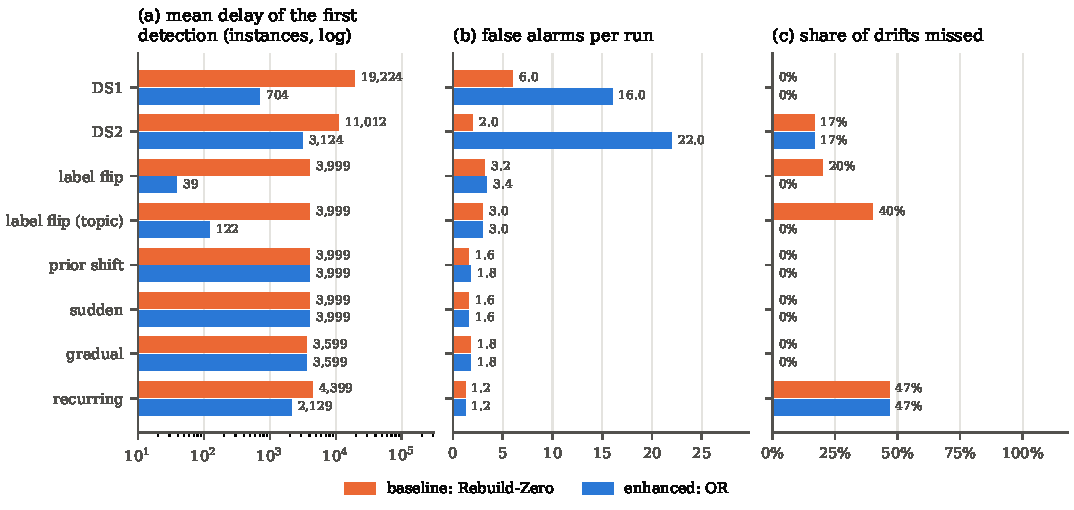
\includegraphics[width=0.92\textwidth]{fig3_detection.pdf}
\caption{Detection per stream for the baseline and the enhanced (OR) model: (a) mean delay of the
first detection, (b) false alarms per run, (c) share of drifts missed.}
\label{fig:detection}
\end{figure*}

\begin{figure*}[!t]
\centering
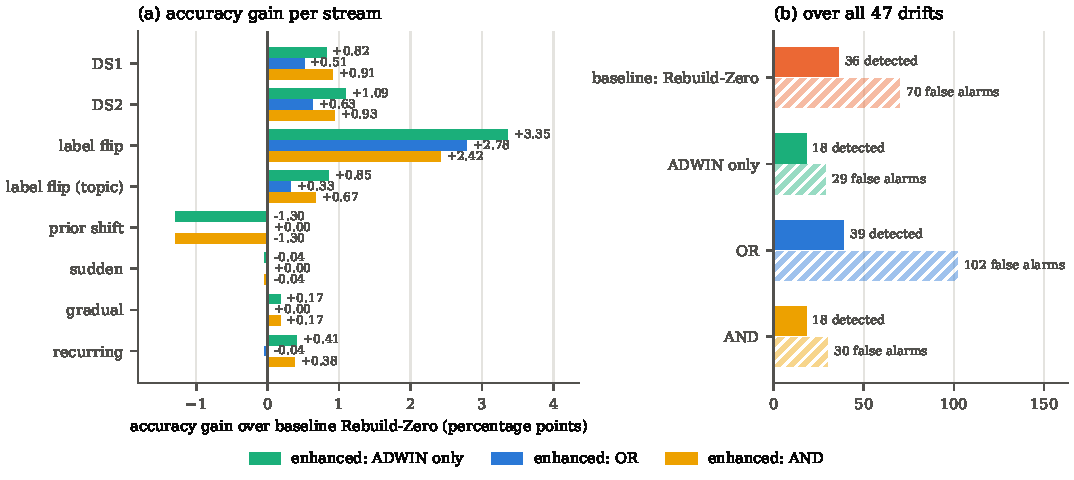
\includegraphics[width=0.92\textwidth]{fig5_ablation.pdf}
\caption{Fusion modes: (a) accuracy gain over the baseline (Rebuild-Zero) per stream; (b)
detected drifts and false alarms over all 47 drifts.}
\label{fig:ablation}
\end{figure*}

\subsection{Baseline Reproduction}
Fig.~\ref{fig:baseline} reproduces the paper's Fig.~2. The ordering holds on both streams:
the accumulative MNB is worst (78.3\% on DS1, 80.3\% on DS2), fixed ageing helps (80.2\%,
82.5\%) and informed strategies reach up to 81.4\% and 83.0\%. After DS1's change point the
adaptive models reach 93--99.9\% while the accumulative MNB stays at 77\%. Two differences from
the paper: our accumulative baseline is about 5 points stronger (paper: about 73\%), and
\emph{-Zero-} variants beat \emph{-Init-} ones, because constant ageing costs 1--2 points in
stable periods. A sweep of the fading $\lambda$ on DS1 (0.02--0.2 per hour) shows no value that
avoids this trade-off (pre-change accuracy 77.8--76.3\%, tail 92--99\%), which supports the
paper's own argument for forgetting only on detected change.

\subsection{Baseline vs.\ Enhancement on Real Drift}
Table~\ref{tab:accuracy} lists accuracy per stream and Table~\ref{tab:main} the main results.
On the label flip (Fig.~\ref{fig:flip}) every model collapses to about 25\% when the labels
invert. The accumulative and fading MNBs never recover within the stream; the baseline stays at
about 25\% until its vocabulary detector fires one window (3{,}999 instances) later, and misses
the flip entirely in one of five seeds. The enhanced model detects the flip after 39 instances,
dips to about 58\%, is back near 70\% about 2{,}000 instances after the flip and reaches 95\% of
its pre-drift level after 3{,}183 instances (baseline: 8{,}204); its accuracy is
$73.8 \pm 0.3\%$ against $71.0 \pm 1.0\%$, with a smaller spread over seeds. When only topic
A's labels invert, the vocabulary detector misses the drift in 2 of 5 runs while ADWIN detects
all five after about 120 instances (Fig.~\ref{fig:detection}). Accuracy rises only from 63.1\%
to 63.5--64.0\% there, because MNB scores words independently and cannot represent a polarity
change limited to one topic: every model is capped at about 64\% after that drift.

\begin{figure}[!t]
\centering
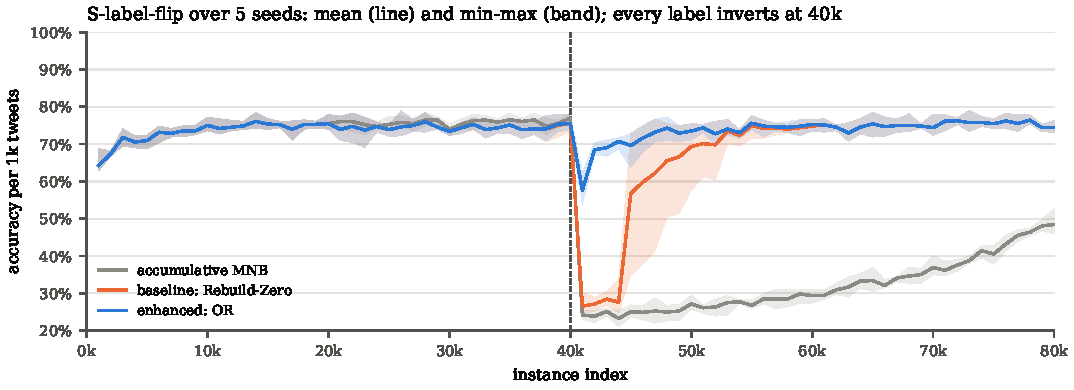
\includegraphics[width=\columnwidth]{fig2_label_flip_seeds.pdf}
\caption{S-label-flip over 5 seeds: mean accuracy per 1k tweets (lines) and min--max over seeds
(bands). All labels invert at 40k.}
\label{fig:flip}
\end{figure}

\subsection{Detection, False Alarms and Recovery}
Over all 47 true drifts (Fig.~\ref{fig:detection}, Table~\ref{tab:main}) the OR model detects 39
with a mean delay of 2{,}290 instances, against 36 and 4{,}766 for the baseline. On DS1 ADWIN
flags the natural change point 704 instances after it, against 19{,}224 for the vocabulary
detector; on DS2 3{,}124 against 11{,}012. The price is false alarms: 102 for OR against 70,
almost all from the vocabulary channel on DS1 and DS2. Recovery (Fig.~\ref{fig:recovery}) is
2.6$\times$ faster on the label flip (3{,}183 vs 8{,}204 instances). On DS1 the enhanced model
never falls below 95\% of its pre-change accuracy, while the baseline needs 2{,}384 instances; on
DS2 the enhanced model recovers slightly more slowly (5{,}560 vs 4{,}610 instances). For the
sudden and gradual topic switches accuracy never falls below the recovery target; on the
recurring scenario both models need 2{,}436 instances, and on all three virtual drifts the
models stay within 0.7 points of each other in accuracy.

\begin{figure}[!t]
\centering
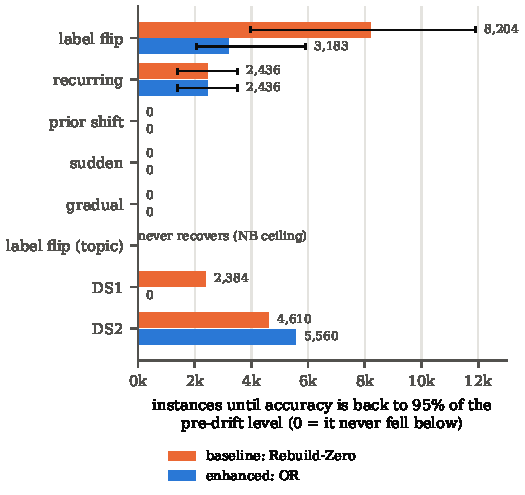
\includegraphics[width=0.85\columnwidth]{fig4_recovery.pdf}
\caption{Recovery time per stream (mean, whiskers: min--max over seeds).}
\label{fig:recovery}
\end{figure}

\subsection{Fusion Modes}
Fig.~\ref{fig:ablation} compares the fusion modes. ADWIN alone gives the largest gains on the
label flips and DS2 and the fewest false alarms (29), but it ignores pure prior shifts and topic
switches because they do not raise the error: on the prior shift it loses 1.3 points, as does
AND. OR keeps the vocabulary channel and with it the prior-shift detection: it never falls more
than 0.04 points below the baseline on any stream, detects the most drifts and matches or beats
the baseline in 28 of 32 stream--seed pairs. We therefore use OR as the main model and report
the others as ablations.

\subsection{Streaming Performance and Cost}
Through Kafka and Spark the two models reproduce the offline accuracies (72\% and 74\% on the
label flip at 1{,}000 tweets/s), and the dashboard shows the enhanced model's ADWIN marker at
the flip while the baseline sits near 25\% (Fig.~\ref{fig:grafana}). With micro-batches capped
at 1{,}000 tweets the pipeline keeps up with 2{,}000 tweets/s at a median latency of 0.42\,s
(p95 0.76\,s) and saturates at about 2{,}840 tweets/s; with a cap of 5{,}000 it sustains
5{,}593 tweets/s at a median latency below 1\,s. The bottleneck is Spark's fixed cost of about
170\,ms per micro-batch, not the models: the baseline needs 22.6\,ms and the enhanced model
32.9\,ms per 1{,}000 tweets (Table~\ref{tab:cost}); ADWIN itself costs under 1\,$\mu$s per
update. Offline, all adaptive models process 37--46k tweets/s.

\begin{figure}[!t]
\centering
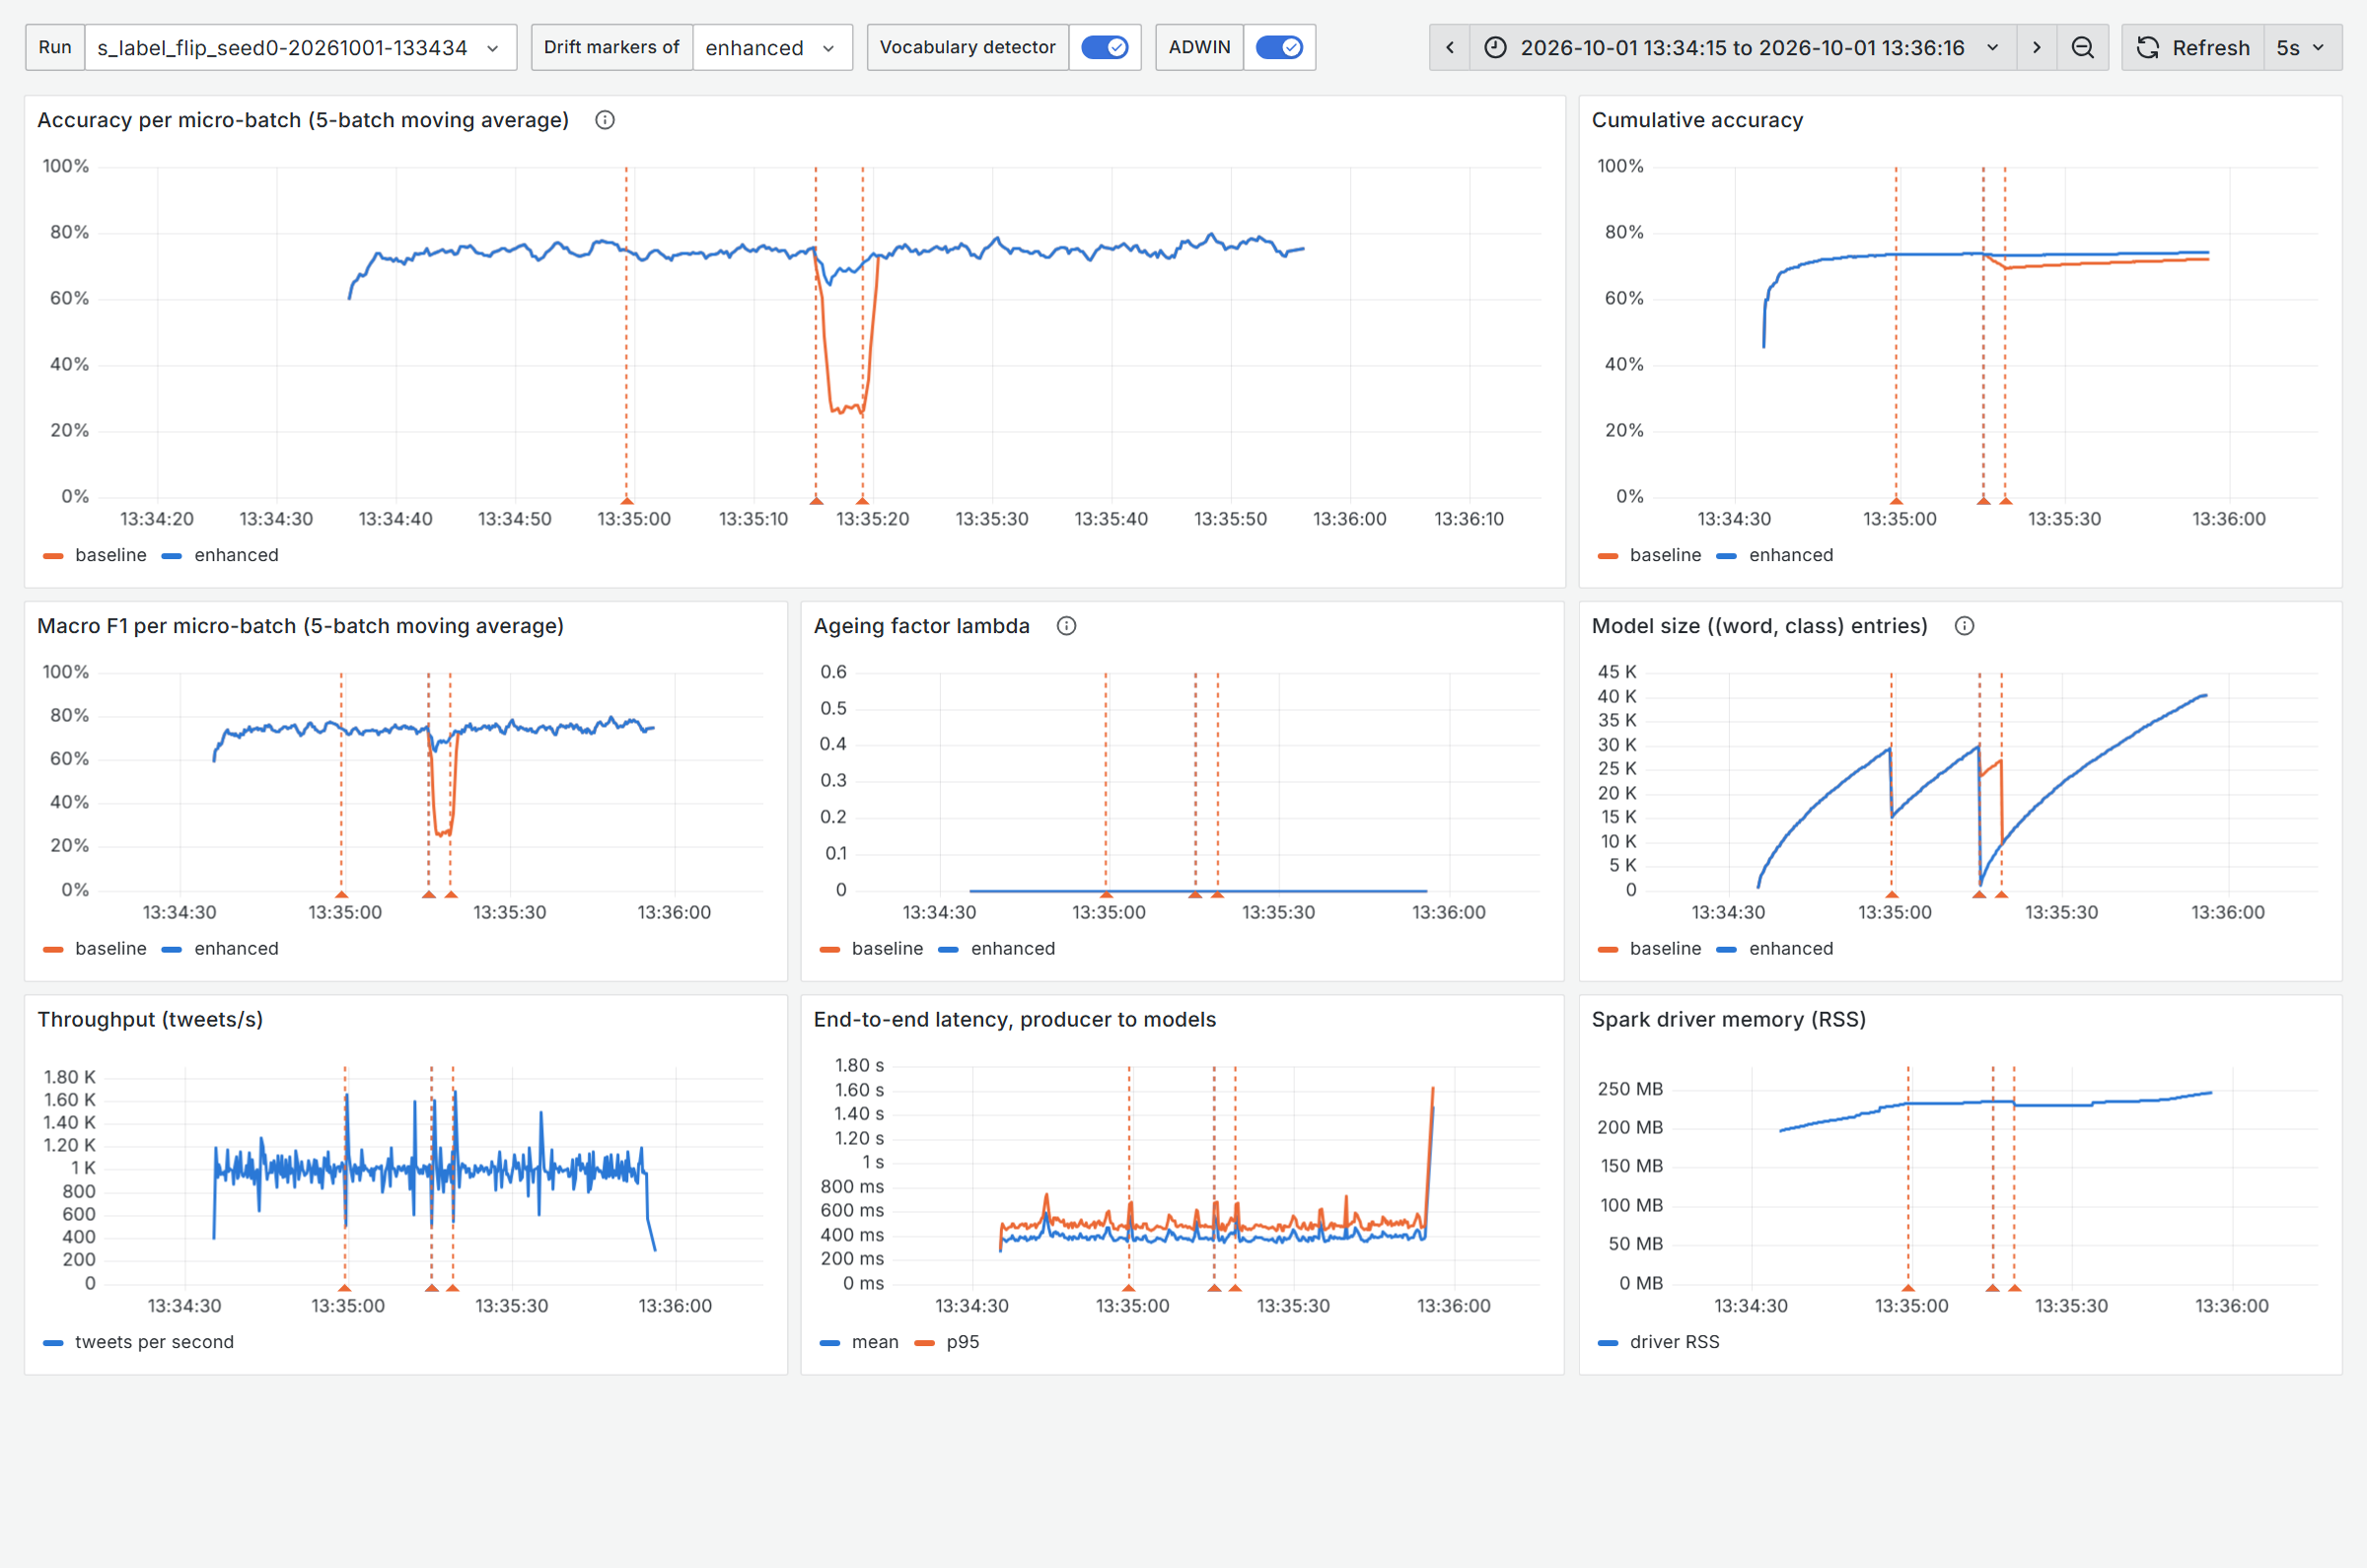
\includegraphics[width=\columnwidth]{grafana_label_flip.png}
\caption{Grafana during a live S-label-flip run (1{,}000 tweets/s): baseline (orange) and
enhanced (blue) side by side, drift annotations (orange: vocabulary detector, blue: ADWIN).}
\label{fig:grafana}
\end{figure}

\begin{table}[t]
\centering
\footnotesize
\caption{Cost of the enhancement. Offline: mean over the grid runs. Spark: model time per 1k tweets in the streaming pipeline (S-label-flip, 1,000 tweets/s); the pipeline adds about 170 ms fixed overhead per micro-batch for both.}
\label{tab:cost}
\resizebox{\linewidth}{!}{%
\begin{tabular}{lrrrr}
\toprule
Model & Offline tweets/s & Batch p50 / p95 (ms) & Entries & Spark ms per 1k \\
\midrule
baseline: Rebuild-Zero & 38,303 & 29 / 55 & 41,934 & 22.6 \\
enhanced: OR & 37,213 & 27 / 58 & 40,088 & 32.9 \\
\bottomrule
\end{tabular}}
\end{table}


\section{Discussion and Inferences}
\textbf{What the results mean.} Monitoring the classifier's error complements monitoring its
input. The vocabulary detector is the right signal for changes in $P(X)$ and $P(y)$ (topic and
prior shifts); ADWIN on the error is the right signal for changes in $P(y\,|\,X)$, and it is
fast because it updates on every tweet rather than every $w$ tweets. Virtual drift barely
affects an MNB classifier, so detecting it is informative but not necessary for accuracy, and an
error-based trigger avoids needless rebuilds. $\lambda$-based strategies depend on the time
scale: SlowIncreaseFastReset is the best baseline on DS1 (81.4\%) but reaches only 54.5\% on the
label flip, because the scenarios span about 22 synthetic hours and a larger $\lambda$ per hour
barely ages the model; rebuilding does not depend on the time unit. Finally, a cheap reaction
makes false alarms cheap: rebuilding from recent data costs little accuracy after a false alarm,
which is why the OR model still gains accuracy despite more false alarms.

\textbf{Limitations.} Sentiment140 labels are derived from emoticons and noisy (1{,}685 tweets
appear with both labels). The models are sequential, so Spark parallelises only ingestion and
tokenisation; the model state lives on the driver and is lost on restart. The data is from 2009,
so vocabulary and usage differ from today's platforms.

\textbf{Threats to validity.} \emph{Internal:} ADWIN's $\delta$ and the vocabulary threshold were
chosen on the same controlled scenarios we evaluate on; the gains on DS1 and DS2, which were not
used for tuning, are smaller but consistent. \emph{Construct:} the controlled drifts are
synthetic and the topics are defined by keywords; the real streams' ground truth contains only
the designed drift points, so their false-alarm counts are upper bounds. \emph{External:} DS2's
removal pattern is our own because the paper does not specify it, and our accumulative baseline
is stronger than the paper's, which narrows the gaps we measure; results on other models or
platforms may differ.

\section{Conclusion and Future Work}
We reproduced informed ageing MNB on Sentiment140 and showed that its vocabulary-based detector
misses or delays drift that changes meaning without changing words. Adding ADWIN on the
prequential error, fused with the vocabulary detector and combined with a rebuild on the
post-drift window, detects such drift about 100 times sooner, recovers 2.6 times faster and
improves accuracy on both real streams at negligible cost, in an end-to-end Kafka, Spark,
InfluxDB and Grafana pipeline. Future work includes a classifier that can model
context-dependent polarity (to lift the naive Bayes ceiling we observed), drift-specific
reactions (e.g.\ reweighting the class prior on a detected prior shift), keyed state so that
Spark can partition the stream across executors, and evaluation on recent, event-driven streams
such as the one studied by Bechini et al.~\cite{bechini2021}.

\bibliographystyle{IEEEtran}
\bibliography{refs}

\end{document}
